%
%===============>>  ГРУППА 11-1 МОДУЛЬ 5  <<=============
%
\setmodule{5}

%BEGIN_FOLD % ====>>_____ Занятие 1 _____<<====
\begin{class}[number=1]
	\begin{listofex}
		\item Занятие 1
	\end{listofex}
\end{class}
%END_FOLD

%BEGIN_FOLD % ====>>_____ Занятие 2 _____<<====
\begin{class}[number=2]
	\begin{listofex}
		%1
		\item Материальная точка движется прямолинейно по закону \(x(t) = 6t^2 - 48t + 17\) (где \(x\)  — расстояние от точки отсчета в метрах, \(t\)  — время в секундах, измеренное с начала движения). Найдите ее скорость (в м/с) в момент времени \(t  =  9\) с.
		%2
		\item Материальная точка движется прямолинейно по закону \(x(t) = -t^4 + 6t^3 + 5t + 23\) (где \(x\)  — расстояние от точки отсчета в метрах, \(t\)  — время в секундах, измеренное с начала движения). Найдите ее скорость в (м/с) в момент времени \(t = 3\) с.
		%3
		\item
		\begin{minipage}[t]{\bodywidth}
			На рисунке изображен график функции \( y = f(x)\), определенной на интервале \((-5; 5)\). Найдите количество точек, в которых касательная к графику функции параллельна прямой \(y  =  6\) или совпадает с ней.
		\end{minipage}
		\hspace{0.02\linewidth}
		\begin{minipage}[t]{\picwidth}
			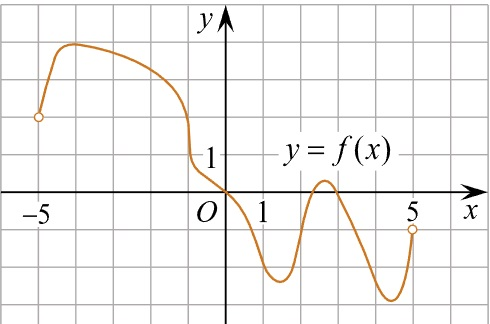
\includegraphics[align=t, width=\linewidth]{\picpath/G111M5L2-1}
		\end{minipage}
		%4
		\item
		\begin{minipage}[t]{\bodywidth}
			На рисунке изображен график производной функции \(f(x)\), определенной на интервале \((-10; 2)\). Найдите количество точек, в которых касательная к графику функции \(f(x)\) параллельна прямой \(y = -2x - 11\) или совпадает с ней.
		\end{minipage}
		\hspace{0.02\linewidth}
		\begin{minipage}[t]{\picwidth}
			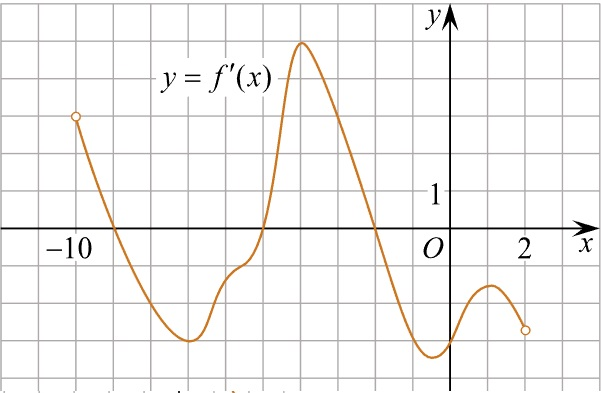
\includegraphics[align=t, width=\linewidth]{\picpath/G111M5L2-2}
		\end{minipage}
		%5
		\item
		\begin{minipage}[t]{\bodywidth}
			На рисунке изображен график производной функции \(f(x)\) , определенной на интервале \( (-6;6) \) . Найдите промежутки возрастания функции \(f(x)\) . В ответе укажите сумму целых точек, входящих в эти промежутки.
		\end{minipage}
		\hspace{0.02\linewidth}
		\begin{minipage}[t]{\picwidth}
			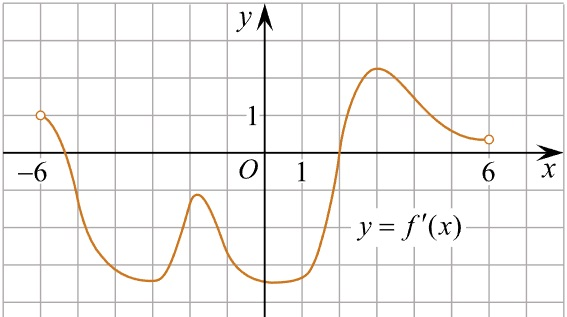
\includegraphics[align=t, width=\linewidth]{\picpath/G111M5L2-3}
		\end{minipage}
		%6
		\item
		\begin{minipage}[t]{\bodywidth}
			На рисунке изображен график функции \(y = f(x)\), определенной на интервале \((-6; 8)\). Определите количество целых точек, в которых производная функции положительна.
		\end{minipage}
		\hspace{0.02\linewidth}
		\begin{minipage}[t]{\picwidth}
			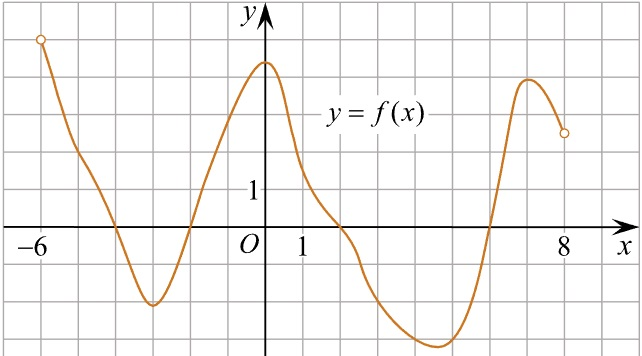
\includegraphics[align=t, width=\linewidth]{\picpath/G111M5L2-4}
		\end{minipage}
		%7
		\item Найдите:
		\begin{itasks}[1]
			\task точку максимума функции \(y = x^3 - 48 + 17\)
			\task наименьшее значение функции \(y = x^3 - 27x\) на отрезке \([0;4]\)
			\task точку максимума функции \(y = x^3 - 5x^2 + 7x -5\)
			\task точку максимума функции \(y = -\dfrac{x^2+289}{x}\)
			\task наименьшее значение функции \(y = \dfrac{x^2+25}{x}\) на отрезке \([1;10]\)
		\end{itasks}
	\end{listofex}
\end{class}
%END_FOLD

%BEGIN_FOLD % ====>>_____ Занятие 3 _____<<====
\begin{class}[number=3]
	\begin{listofex}
		\item В треугольнике \(ABC\) угол \(C\) равен \(90 \degree \), \(AC=4,8\), \(\sin{A} = \dfrac{\sqrt{17}}{17}\). Найдите \(BC\).
		\item В треугольнике \(ABC\) угол \(C\) равен \(90 \degree \), \(AC=2\), \(\cos{A} = 0,5\). Найдите \(AB\).
		\item В треугольнике \(ABC\) угол \(C\) равен \(90 \degree \), \(AC=4\), \(\tan{A} = \dfrac{33}{4\sqrt{33}}\). Найдите \(AB\).
		\item В треугольнике \(ABC\) угол \(C\) равен \(90 \degree \), \(AC=4\), \(BC=7\). Найдите \(\sin{A}\).
		\item В треугольнике \(ABC\) угол \(C\) равен \(90 \degree \), \(CH\) --- высота, \(AB=13\), \(\tan{A} = 5\). Найдите \(BH\).
		\item В треугольник \(ABC, AC = BC = 5\), \( \sin{A}= \dfrac{7}{25} \). Найдите \(AB\).
		\item В треугольник \(ABC, AC = BC, AB = 8\), \( \cos{A}= 0,5 \). Найдите \(AC\).
		\item В треугольник \(ABC, AC = BC = 7\), \( \tg{A}= \dfrac{33}{4 \cdot \sqrt[]{33}} \). Найдите \(AB\).
	\end{listofex}
\end{class}
%END_FOLD

%BEGIN_FOLD % ====>>_____ Занятие 4 _____<<====
\begin{class}[number=4]
	\begin{listofex}
		\item В треугольнике \(ABC\) угол \(C\) равен \(90 \degree \), \(AC=4,8\), \(\sin{A} = \dfrac{7}{25}\). Найдите \(AB\).
		\item В треугольнике \(ABC\) угол \(C\) равен \(90 \degree \), \(AC=2\), \(\cos{A} = \dfrac{\sqrt{17}}{17}\). Найдите \(AC\).
		\item В треугольнике \(ABC\) угол \(C\) равен \(90 \degree \), \(AC=8\), \(\tan{A} = 0,5\). Найдите \(AB\).
		\item В треугольнике \(ABC\) угол \(C\) равен \(90 \degree \), \(CH\) --- высота, \(AB=13\), \(\tan{A} = \dfrac{1}{5}\). Найдите \(AH\).
		\item В треугольнике \(ABC\) угол \(C\) равен \(90 \degree \), \(CH\) --- высота, \(BC=3\), \(\sin{A} = \dfrac{1}{6}\). Найдите \(AH\).
		\item В треугольник \(ABC, AC = BC, AB = 9,6\), \( \sin{A}= \dfrac{7}{25} \). Найдите \(AC\).
		\item В треугольник \(ABC, AC = BC = 8\), \( \cos{A}= 0,5 \). Найдите \(AB\).
		\item В треугольник \(ABC, AC = BC, AB = 8\), \( \tg{A}= \dfrac{33}{4 \cdot \sqrt[]{33}} \). Найдите \(AC\).
	\end{listofex}
\end{class}
%END_FOLD

%BEGIN_FOLD % ====>>_____ Занятие 5 _____<<====
\begin{class}[number=5]
	\begin{listofex}
		\item Занятие 5
	\end{listofex}
\end{class}
%END_FOLD

%BEGIN_FOLD % ====>>_____ Занятие 6 _____<<====
\begin{class}[number=6]
	\begin{listofex}
		\item Занятие 6
	\end{listofex}
\end{class}
%END_FOLD

%BEGIN_FOLD % ====>>_____ Занятие 7 _____<<====
\begin{class}[number=7]
	\begin{listofex}
		\item Занятие 7
	\end{listofex}
\end{class}
%END_FOLD

%BEGIN_FOLD % ====>>_ Домашняя работа 1 _<<====
\begin{homework}[number=1]
	\begin{listofex}
		%1
		\item Материальная точка движется прямолинейно по закону \(x(t) = t^2 - 13t + 23\) (где \(x\)  — расстояние от точки отсчета в метрах, \(t\)  — время в секундах, измеренное с начала движения). В какой момент времени (в секундах) ее скорость была равна \(2\) м/с?
		%2
		\item
		\begin{minipage}[t]{\bodywidth}
			На рисунке изображён график \(y=f'(x)\)   — производной функции \(f(x)\)  , определенной на интервале \((-8; 3)\). В какой точке отрезка \([-3; 2]\) функция \(f(x)\) принимает наибольшее значение?
		\end{minipage}
		\hspace{0.02\linewidth}
		\begin{minipage}[t]{\picwidth}
			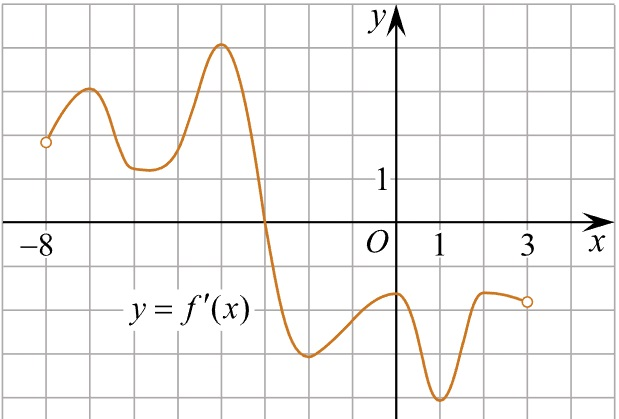
\includegraphics[align=t, width=\linewidth]{\picpath/G111M5H1-1}
		\end{minipage}
		%3
		\item
		\begin{minipage}[t]{\bodywidth}
			На рисунке изображен график производной функции \(f(x)\), определенной на интервале \((-8; 4)\). В какой точке отрезка \([-7; -3] f(x)\) принимает наименьшее значение?
		\end{minipage}
		\hspace{0.02\linewidth}
		\begin{minipage}[t]{\picwidth}
			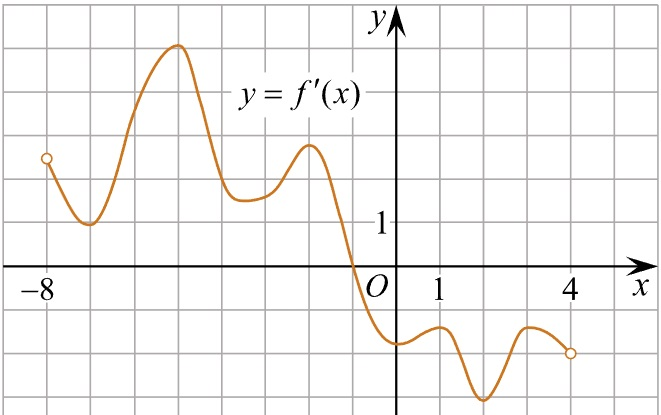
\includegraphics[align=t, width=\linewidth]{\picpath/G111M5H1-2}
		\end{minipage}
		%4
		\item
		\begin{minipage}[t]{\bodywidth}
			На рисунке изображён график функции \(y=f(x)\) и касательная к нему в точке с абсциссой \(x_0\). Найдите значение производной функции \(f(x)\) в точке \(x_0\).
		\end{minipage}
		\hspace{0.02\linewidth}
		\begin{minipage}[t]{\picwidth}
			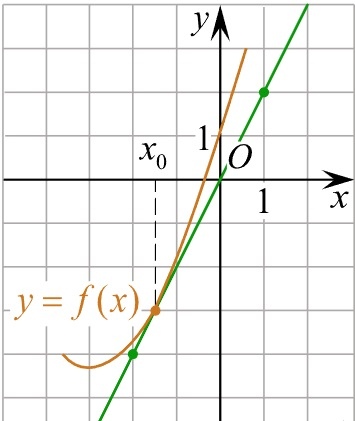
\includegraphics[align=t, width=\linewidth]{\picpath/G111M5H1-3}
		\end{minipage}
		%5
		\item
		\begin{minipage}[t]{\bodywidth}
			На рисунке изображены график функции \(y = f(x)\) и касательная к нему в точке с абсциссой \(x_0\). Найдите значение производной функции \(f(x)\) в точке \(x_0\).
		\end{minipage}
		\hspace{0.02\linewidth}
		\begin{minipage}[t]{\picwidth}
			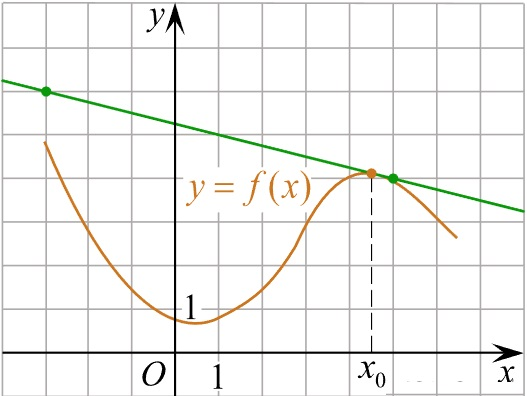
\includegraphics[align=t, width=\linewidth]{\picpath/G111M5H1-4}
		\end{minipage}
		%6
		\item Найдите:
		\begin{itasks}[1]
			\task точку максимума функции \(y = x^3 - 3x^2 + 2\)
			\task наименьшее значение функции \(y = x^3 - 6x^2\) на отрезке \([0;4]\)
			\task точку максимума функции \(y = x^3 + 2x^2 + x + 5\)
			\task точку максимума функции \(y = -\dfrac{x^2+1}{x}\)
			\task наименьшее значение функции \(y = x + \dfrac{36}{x}\) на отрезке \([1;9]\)
			\task точку максимума функции \( y=-\dfrac{x}{x^2+289} \)
		\end{itasks}
	\end{listofex}
\end{homework}
%END_FOLD

%BEGIN_FOLD % ====>>_ Домашняя работа 2 _<<====
\begin{homework}[number=2]
	\begin{listofex}
		\item В треугольнике \(ABC\) угол \(C\) равен \(90 \degree \), \(CH\) --- высота, \(BC = 8\), \(\sin{A} = 0,5\). Найдите \(BH\).
		\item В треугольнике \(ABC\) угол \(C\) равен \(90 \degree \), \(CH\) --- высота, \(BC=3\), \(\cos{A} = \dfrac{\sqrt[]{35}}{6}\). Найдите \(AH\).
		\item В треугольнике \(ABC\) угол \(C\) равен \(90 \degree \), \(CH\) --- высота, \(BC=5\), \(\cos{A} = \dfrac{7}{25}\). Найдите \(BH\).
		\item В треугольник \(ABC, AC = BC, AB = 8\), \( \sin{BAC}= 0,5 \). Найдите высоту \(AH\).
		\item В треугольник \(ABC, AC = BC, AB = 8\), \( \cos{BAC}= \dfrac{7}{25} \). Найдите высоту \(AH\).
		\item В треугольник \(ABC, AC = BC\), \(AH\) --- высота \( \cos{BAC}= 0,5 \). Найдите высоту \(BH\).
	\end{listofex}
\end{homework}
%END_FOLD

%BEGIN_FOLD % ====>>_ Домашняя работа 3 _<<====
\begin{homework}[number=3]
	\begin{listofex}
		\item ДЗ 3
	\end{listofex}
\end{homework}
%END_FOLD

%BEGIN_FOLD % ====>>_ Проверочная работа _<<====
\begin{exam}
	\begin{listofex}
		\item Проверочная работа
	\end{listofex}
\end{exam}
%END_FOLD
